\documentclass{beamer}
\setbeamercovered{highly dynamic}
\usepackage[utf8]{inputenc}
\usepackage[T1]{fontenc}
\usepackage{lmodern}
\usetheme{Madrid}
\usepackage{tikz}
\usetikzlibrary{automata, positioning, arrows}

\tikzset{
	node distance=3cm, % specifies the minimum distance between two nodes. Change if necessary.
	every state/.style={thick, fill=gray!10}, % sets the properties for each ’state’ node
	initial text=$ $, % sets the text that appears on the start arrow
}


\title{Metodologia de Pesquisa}
\subtitle{Simulação}
\author{Ricardo Rosal}
\begin{document}
	\begin{frame}[plain]
	\maketitle
	\end{frame}	
	\begin{frame}
		\tableofcontents
	\end{frame}
	\section{Simulação como método de pesquisa}
		\subsection{O que é simulação?}
		isso é um modelo...
	
	
	\subsection{Porque fazer uma simulação?}
	\subsection{Vantagens da simulação}
	
	\begin{frame}{Simulação como método de pesquisa}
		\begin{itemize}[<+->]
			\item O principal valor da simulação como método de pesquisa é a flexibilidade dada ao pesquisar de focar na complexidade do sistema e do modelo em estudo e fazer perguntas do tipo \textbf{"e se?"} ao ínves de perguntas como \textbf{"o que aconteceu? como? e por que?"}.
			\item outros métodos de pesquisa, em contra-partida, requer que seja \textbf{estabelescida algumas preposições sobre causalidade do fenômeno estudado}, já a simulação nos permite, desde a dinâmica estabelescida do modelo, \textbf{"criar/descobrir"} tais efeitos e demostrar causalidades.
			\item A simulação permite o estudo de \textbf{fenômenos mais complexos}, uma vez que as observações são feitas para \textbf{"avançando"} no tempo (ou em outro dimensão em que o sistema tem uma dinâmica definida).
		\end{itemize}
	\end{frame}
	\subsection{Tipos de simulação}
	\subsubsection{Eventos discretos}
	\begin{frame}{Principais familias de simulação}
		\begin{itemize}[<+->]
			\item \textbf{Simulação de eventos discretos:} envolve um modelo onde a dinâmica (\emph{governing equations}) na dimensão $\zeta$ (tempo, por exemplo) evolui de forma discreta, normalmente os eventos são disparados por um gatilho, que pode ser implementado com uma \textbf{callback} ou um \textbf{intervalo pré-definido}.
			\item usalmente, metódos como maquinas de \textbf{estados-finitos}, e \textbf{teoria das filas} são utilizados para simulação de eventos discretos.
			\item exemplo:
			\centering
				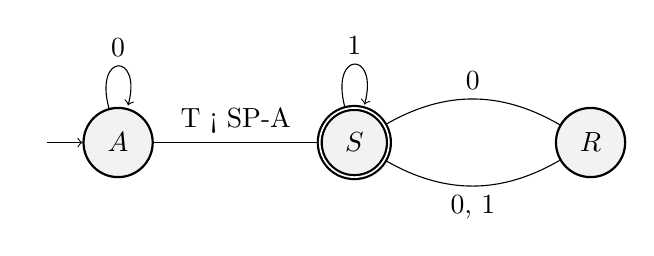
\begin{tikzpicture}
					\node[state, initial] (q1) {$A$};
					\node[state, accepting, right of=q1] (q2) {$S$};
					\node[state, right of=q2] (q3) {$R$};
					\draw 	(q1) edge[loop above] node{0} (q1)
							(q1) edge[above] node{T < SP-A} (q2)
							(q2) edge[loop above] node{1} (q2)
							(q2) edge[bend left, above] node{0} (q3)
							(q3) edge[bend left, below] node{0, 1} (q2);
				\end{tikzpicture}	
		\end{itemize}

	\end{frame}
	\subsubsection{Sistemas dinâmicos}
	\begin{frame}{Principais familias de simulação}
		\begin{itemize}[<+->]
			\item \textbf{Simulação de sistemas dinâmicos:} nesse tipo de simulação é definido o \textbf{estado} ou \textbf{estados} do sistema, que normalmente é a variável dependente de uma função, onde é conhecido a dinâmica do mesmo.
			\item essa dinâmica normalmente é definida por uma \textbf{equação diferencial} \textbf{ODE} ou \textbf{PDE}, dependendo do número de \textbf{dimensões} no espaço onde ocorre a dinâmica do sistema, e a função que define o \textbf{estado} é a solução da equação diferencial.
			\item Por exemplo:
			\begin{equation}
				F = m \cdot a
			\end{equation}			
			\begin{equation}
				m\frac{d^2x}{dt^2} - f = 0
			\end{equation}
			\item ou:
			\begin{equation}
				\nabla^2=\frac{\rho}{\varepsilon}
			\end{equation}
		\end{itemize}
	\end{frame}
	\subsubsection{Simulação baseada em agentes}
	\begin{frame}{Principais familias de simulação}
		\begin{itemize}[<+->]
			\item \textbf{Simulaçãos baseadas em agentes:} são um grupo de metodos que de simulação que tem como objetivo a iteração de agentes que tendem a otimizar suas \textbf{funções de utilidade}.
			\item Um dos metodos mais utilizados para esse tipo de simulação a \textbf{teoria dos jogos}.
		\end{itemize}
	\end{frame}
	\section{Os objetivos de uma simulação}
	\subsection{Predição}
	\begin{frame}{Simulação como previsão}
		\begin{itemize}
			\item As simulações partem de um modelo composto por \textbf{governing rules} e \textbf{constitutive relations} e produz \textbf{saídas} dessas regras.
			\item Comparando as diferentes saidas de diferentes modelos e parâmetros que constituem os modelos, os pesquisadores podem inferir a relação de dado parâmetro no comportamento da saída.
			\item A validade dessas dependem intrísicamente da validade do modelo.
			
		\end{itemize}
	\end{frame}
	\section{Métodos de simulação}
		\subsection{Sistemas dinâmicos}
		\begin{frame}{O que é um sistema dinâmico?}
			\begin{itemize}[<+->]
				\item Em resumo, um \textbf{sistema dinâmico} é um sistema que varia no tempo;
				\item o sistema é descrito uma variavel que define o estado do sistema;
					\begin{equation}
						s(t)
					\end{equation}
				\item o estado pode ser um vetor (multivariavel);
					\begin{equation}
						s(t)=(s(t),...,s_n(t))^{T}
					\end{equation}
				\item e para adicionar a \emph{dinâmica} no sistema, é necessário definir como o \textbf{estado} varia no tempo.
				\item qual a forma mais convencional de fazer isso matematicamente?
				\begin{equation}
					\dot{s}(t) = \frac{s(t)}{dt} = f(s(t))
				\end{equation}
			\end{itemize}
		\end{frame}
		\begin{frame}{Representações de sistemas dinâmicos}
			\par Temos geralmente duas formas de representar o tempo em sistemas dinâmicos, e isso normalmente depende da dinâmica do sistema e como isso será definido.
			\begin{itemize}[<+->]
				\item \textbf{Tempo discreto:} os tempo nos sistemas dinâmicos são representados \textbf{relações recorrentes} tambem chamado de \textbf{equações de diferenças}.
				\begin{equation}
					s(t+\Delta t) = f(s(t))
				\end{equation}
				\item \textbf{Tempo continuo:} já nos sistemas contínuos são representados por \textbf{equações diferenciais}, ordinárias (ODE) ou parciais (PDE).
				\begin{equation}
					\dot{s} = \frac{ds(t)}{dt} = f(s(t))
				\end{equation}			
			\end{itemize}
		\end{frame}
		\begin{frame}{Exemplo: Crescimento Populacional}
			\begin{itemize}[<+->]
				\item Vamos abordar um problema onde aplicação onde o objeto é simular o \textbf{"crescimento"} de uma população em um dado sistema.
				\item podemos começar modelando esse sistema, definindo a variável estado do sistema, que no caso é a população $P(t)$.
				\item Considerando que sabemos o estado atual da população $P(0)=P_0$, temos um IVP.
				\item De forma bastante resumida, podemos falar que os unicos processos que influenciam o estado da população é a $M(t)$ e o nascimento $N(t)$.
				\item então podemos definir que:
					\begin{equation}
						\dot{P}= \frac{P(t)}{dt} = N(t)-M(t)
					\end{equation}
				\item Possiveis funções para modelar os nascimentos e mortes poderiam ser:
					\begin{equation}
						B(t)=r_bP(t)
					\end{equation}
					\begin{equation}
						B(t)=r_dP(t)
					\end{equation}
			\end{itemize}
		\end{frame}
		\begin{frame}{Exemplo: Crescimento Populacional}
			\begin{itemize}[<+->]
				\item Podemos simplificar esse problema da seguinte forma:
					\begin{equation}
						\dot{P}=rP(t) \text{ onde } r=rb-rd
					\end{equation}
				\item E, por ser um modelo \textbf{muito} simples, podemos resolve-lo analiticamente.
					\begin{equation}
						P(t)=P_0e^{rt}
					\end{equation}
			\end{itemize}
		\end{frame}
		\subsection{Monte Carlo}
		\begin{frame}{O que é metodo de Monte Carlo?}
			\begin{itemize}[<+->]
				\item O objetivo do metodo de monte de carlo é amostrar um processo estocástico e a partir disso, determinar propriedades estatísticas do fenomeno.
				\item no entanto, como é amostrado os eventos aleatórios?
				\item A principal sacada do metodo de Monte Carlo foi utlizar a função inversa de uma CDF (cumulative distribution function) para, a partir de um gerador de numeros aleatórios, definir o estado do evento gerado.
				\item Por exemplo, se jogarmos uma moeda 4 vezes, qual é a probabilidade de obtermos 3 caras e 1 coroa?
				\item podemos definir isso analiticamente pelo seguinte processo (distribuição binomial):
				\begin{equation}
					P(3 caras) = \binom{4}{3}\frac{1}{2}^2\big(1-\frac{1}{2})^1 = \frac{1}{4}
				\end{equation}
			\end{itemize}
		\end{frame}
		\subsection{Elementos Finitos}
		\subsection{CPS (Cyber-Phyisical System)}
		\subsection{Automatos Celulares}
		\subsection{Lattice Boltzmann}
		\subsection{Point-like object}`
	\section{Abordagens de simulação}
	\section{Implementação de uma simulação}
	\section{Conclusão}
\end{document}
